\documentclass{beamer}

\usetheme{Boadilla}


\usepackage{colortbl}
\usepackage{multimedia}
\usepackage{comment}
\usepackage{graphics}
\usepackage{algorithm}
\usepackage{algpseudocode}
\usepackage{amsmath}


\definecolor{pink}{rgb}{0.8,0.6,0.6}
\definecolor{blue}{rgb}{0.2,0.2,0.8}
\setbeamertemplate{frametitle}[default][center]
\setbeamertemplate{navigation symbols}{}
\setbeamercolor{item}{fg=red}
\setbeamertemplate{items}[square]


%% Macro
\def\x{\mathbf{x}}
\def\R{\mathbb{R}}
\def\n{\mathbf{n}}
\def\bbeta{\boldsymbol\beta}
%%


\begin{document}

\title{A simple approach to mesh deformation}
\author{Shingo Ito}
%\institute{s1200045}
\date{}

\frame{\titlepage}
%% page 1 : title


\begin{frame}
\frametitle{Table of contents} 
\Large
\begin{enumerate}
\item Introduction
\item Related works
\item Algorithm overview
\item Algorithm and implementation details
\item Experiments and result
\item Conclusion

\end{enumerate}
\end{frame}


%page2
\section{Introduction}


\begin{frame}
	\frametitle{Introduction}
	\Large
	\begin{itemize}
	\item Surface deformation is an important research topic in shape and geometric modeling.
   	\item Here we present a simple approach for mesh deformation based on surface reconstruction of a deformed sampled point-cloud.
	\end{itemize}
	%\end{block}
\end{frame}

%page3
\section{Related works}
\begin{frame}
\frametitle{Related works}
\Large
\begin{itemize}
\item Mesh deformation through variational principles (as solution of the harmonic, biharmonic or polyharmonic equation),
\item Cage-based deformation (using generalized barycentric coordinates),
\item Computing the distance to the surface and deforming this distance field (level-set methods).
\end{itemize}
\end{frame}

%page4
\section{Algorithm overview}
\begin{frame}
	\frametitle{Algorithm overview}

\begin{algorithm}[H]
\caption{Overview}
\begin{algorithmic}
\State{Sample from the surface}
\State{Apply the deformation field to the samples}
\State{Apply a surface reconstruction algorithm to the samples}
\end{algorithmic}
\end{algorithm}

\end{frame}


%page5
\section{Algorithm and implementation details}

\begin{frame}
\frametitle{Surface sampling}

\begin{algorithm}[H]
\caption{Uniform sampling from a triangle}
\label{alg:sample}
\begin{algorithmic}
\Function{Sample}{$p_1$, $p_2$, $p_3$, $\xi_1$, $\xi_2$}

\Comment{$p_1$, $p_2$ and $p_3$ are the triangle vertices, 
$\xi_1$ and $\xi_2$ are samples from the unit uniform distribution}

\State Compute the barycentric coordinates: $u = 1-\sqrt{\xi_1}$ 
and $v = \xi_2 \sqrt{\xi_1}$
\State Compute the sample: $P = u * p_1 + v * p_2 + (1 - u - v) * p_3$

\Return $P$
\EndFunction
\end{algorithmic}
\end{algorithm}

\end{frame}


\begin{frame}
	\frametitle{Points deformation}
	\Large
		Given a selected vertex $x_S$ from the input surface, 
		apply to each point a truncated Gaussian centered on this selected vertex
		in the normal direction:
\[f(x)=
\begin{cases}
 \frac{1}{\sqrt{2\pi \sigma^2}} \exp \left(- \frac{(\x- \x_S)^{2}}{2 \sigma^{2}}\right) & \text{if } \|\x-\x_S\| < r \\
0 & \text{otherwise}
\end{cases}
\]
where $r$ is the radius of influence for the truncated Gaussian.

\end{frame}


\begin{frame}
	\frametitle{Surface reconstruction}
	\Large
	Implementation and experiments with three surface reconstruction algorithms.\\
	All approaches are implicit surface based surface reconstruction algorithms. I.e. the output is a function $f$:\\
	\[f: \R^3 \rightarrow \R\]
	The zero level-set of $f$ corresponds to the surface of interest.
\end{frame}


\begin{frame}
	\frametitle{Hermite Radial Basis Functions (Macedo et al.)}
\Large
Given a set of points $P = {\x_i}$ with normal vector at each point $N = {\n_i}$, 
look for a function: $f : \R^3 \to \R$ defined as follows:
\[
f(\x)=\sum_{i=1}^n(\alpha_i\phi(\|\x-\x_i\|)-\bbeta_i\nabla\phi(\|\x-\x_i\|))
\]
where the unknowns to be determined are the coefficients $\alpha_i$ and $\bbeta_i$.

\end{frame}


\begin{frame}
\frametitle{Hermite Radial Basis Functions}
\Large
The conditions used to determine the coefficients are: \[f(\x_i) = 0, \x_i \in \R^3\]
for interpolating points on the surface. And: \[\nabla f(\x_i)=\n_i, \x_i \in \R^3, \n_i \in \R^3\]
for interpolating the normals on the surface.
\end{frame}


\begin{frame}
\frametitle{Hermite Radial Basis Functions}
\Large
This gives the following system of equations to solve:
\[f(\x_i)=\sum_{j=1}^n(\alpha_j\phi(\|\x_i-\x_j\|)-\bbeta_j\nabla\phi(\|\x_i-\x_j\|))=0\]
\[\nabla f(\x_i)=\sum_{j=1}^n(\alpha_j\nabla\phi(\|\x_i-\x_j\|)-H\phi(\|\x_i-\x_j\|)\bbeta_j)=\n_i\]
where $H$ is the Hessian matrix of $\phi$.
\end{frame}


\begin{frame}
	\frametitle{Hermite Radial Basis Functions}
	\Large
	Adding linear polynomials and the additional condition:
	\begin{equation} \label{hrbfcond}
	\sum_{j=1}^n[p_k(x_j)\nabla p_k(x_j)^T]\begin{bmatrix}\alpha_j\\\bbeta_j\end{bmatrix}=0
	\end{equation}
	We obtain:
	\begin{align} \label{hrbf1}
 & \sum_{j=1}^n
\begin{bmatrix}
\phi(\|\x_i-\x_j\|) & -\nabla\phi(\|\x_i-\x_j\|)^T\\ \nabla\phi(\|\x_i-\x_j\|) & -H\phi(\|\x_i-\x_j\|)
\end{bmatrix}
\begin{bmatrix}
\alpha_j\\\bbeta_j
\end{bmatrix} \nonumber
\\
 & + \sum_{l=1}^m\lambda_l
\begin{bmatrix}
p_l(\x_i)\\\nabla p_l(\x_i)
\end{bmatrix}
=
\begin{bmatrix}
0 \\ \n_i
\end{bmatrix}
\end{align}
%\]

\end{frame}


\begin{frame}
	\frametitle{Hermite Radial Basis Functions}
	\Large
	One possible choice of basis function is the triharmonic splines:
	\[ \phi(\|\x\|) = \|\x\|^3 \]
\[\nabla\phi(\|\x\|) = 3\x\|\x\|\]
\[ H \phi (\|\x\|)= \left\{ \begin{array}{ll} 3/\|\x\|(\|\x\|^2I_{3\times3}) + \x\x^T, & \|\x\| \neq 0\\ 
0_{3\times3}, &\|\x\| = 0 \end{array}\right.\]
\end{frame}


\begin{frame}
\frametitle{Closed form approximation for compactly supported functions (Liu and Wang)}

When compactly supported functions are used, 
it is possible to compute an approximation to the solution 
without forming or inverting any matrix
\begin{equation} \label{hrbfclosed}
f(x)=-\sum_{j=1}^n<\frac{\rho^2_j}{20+\eta\rho^2_j} \n_j, \nabla\phi_{\rho_j}(\|\x-\x_j\|)>
\end{equation}
where $\rho_j$ is the radius of support of the basis function associated to the center $j$, 
and $\phi$ is the compactly supported basis function. 
\[
\phi_{\rho}(r)=\phi(r/\rho)
\]
where:
\[
\phi (t)= \left\{ \begin{array}{ll} (1-t)^{4}(4t+1), & t \in [0,1]\\ 
0, & \text{otherwise} \end{array}\right.
\]

\end{frame}


\begin{frame}
	\frametitle{Poisson surface reconstruction (Kazhdan, Bolitho and Hoppe)}
\Large
The third approach consists in computing an indicator function for the solid 
to be reconstructed:
\[
f_S (\x)= \left\{ \begin{array}{ll} 1 & \x \in S\\ 
0 & otherwise \end{array}\right.
\]\\
by solving the Poisson equation
\[
\Delta f=div(\n)
\]
where $\n$ is an extrapolation of the given normal vector field.
\end{frame}


\begin{frame} 
\frametitle{Meshing}
\Large
To recover a triangle mesh for the deformed point-cloud and the corresponding function $f$,
its zero level-set needs to be meshed.
\\
Two approaches were used:
\begin{itemize}
\item Marching Cubes
\item Delaunay based approach
\end{itemize}
\end{frame}


\begin{frame}
\frametitle{Marching Cubes (Lorensen and Cline)}
Algorithm for rendering isosurfaces from volumetric data. \\
\begin{itemize}
\item Compute a bounding box for the object to be meshed and subdivide it regularly into smaller cells. 
\item Sample the function f at the eight corners of each cell.
\item If one or more values is less than the user-specified iso-value, and one or more have values is greater than this isovalue, the cell must intersect the isosurface.
\item Determine the edges in the cell that are intersected by the isosurface.
\item Connect the patches from all cells, we get a linear approximation of the isosurface.
\end{itemize}
\end{frame}


\begin {frame}
\frametitle{Delaunay based implicit surface meshing}
\Large
Marching Cubes based algorithm sample the function at each cells node. 
But it does not exploit the information about the surface location. Instead 
it seems preferrable to use the following approach:
\begin{itemize}
\item Compute a Delaunay tetrahedralization of the deformed point-cloud.\\
\item Peel off outside tetrahedra using the fitted function\\
\end{itemize}
\end{frame}


\section{Experiments and result}

\begin{frame}
\frametitle{The environment used for prototype and in the experiments}
\Large
The development and all experiments were run on a regular note PC. \\
\begin{table}
\begin{center}
\begin{tabular}{|p{3cm}|p{7cm}|} 
\hline
CPU & Intel Corei5 1.4GHz \\ 
\hline
GPU & Intel HD Graphics5000 \\ 
\hline
Memory & 4.0GB RAM \\ 
\hline
OS & OS X Yosemite version 10.10.5 \\  
\hline
Programming Language & C++ \\
\hline 
Libraries & CGAL4.7, OpenGL, Eigen \\ 
\hline
\end{tabular}
\end{center}
\end{table}

\end{frame}


\begin{frame}
	\frametitle{Deformation of a sphere}
 Start from a sphere represented by a triangle mesh, made of 174 vertices and 344 triangles. \\
 \begin{figure}
 \centering
 \hbox{
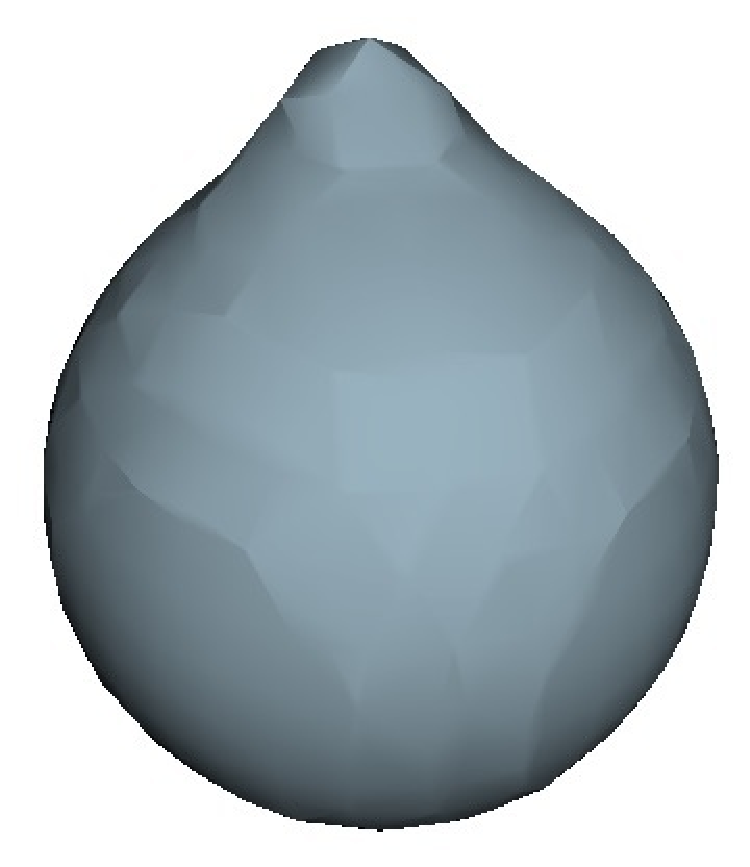
\includegraphics[width=0.30\columnwidth]{deformedspherehrbf.eps}
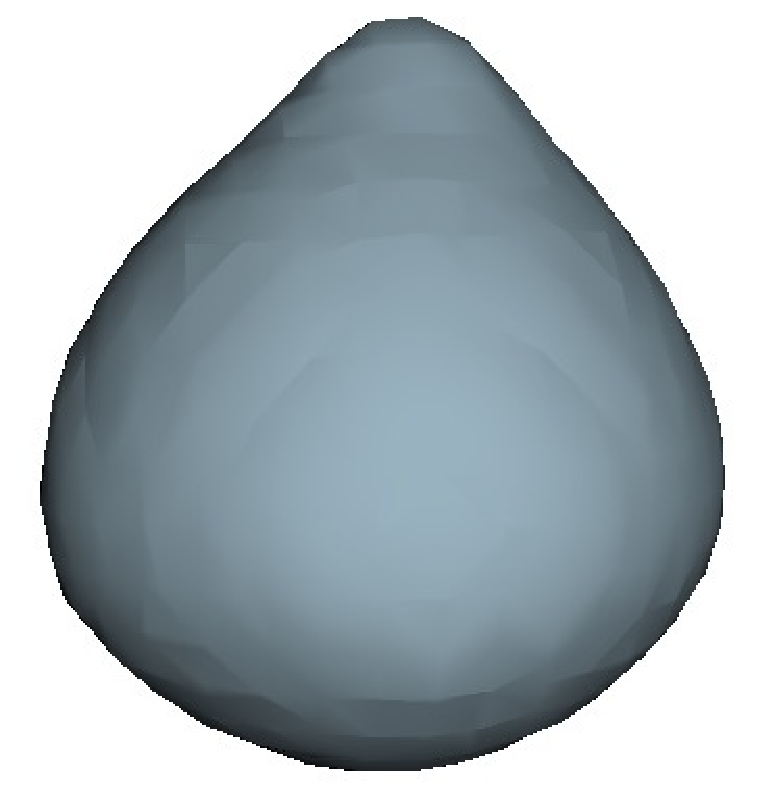
\includegraphics[width=0.30\columnwidth]{deformedspherehrbfclosed3.eps}
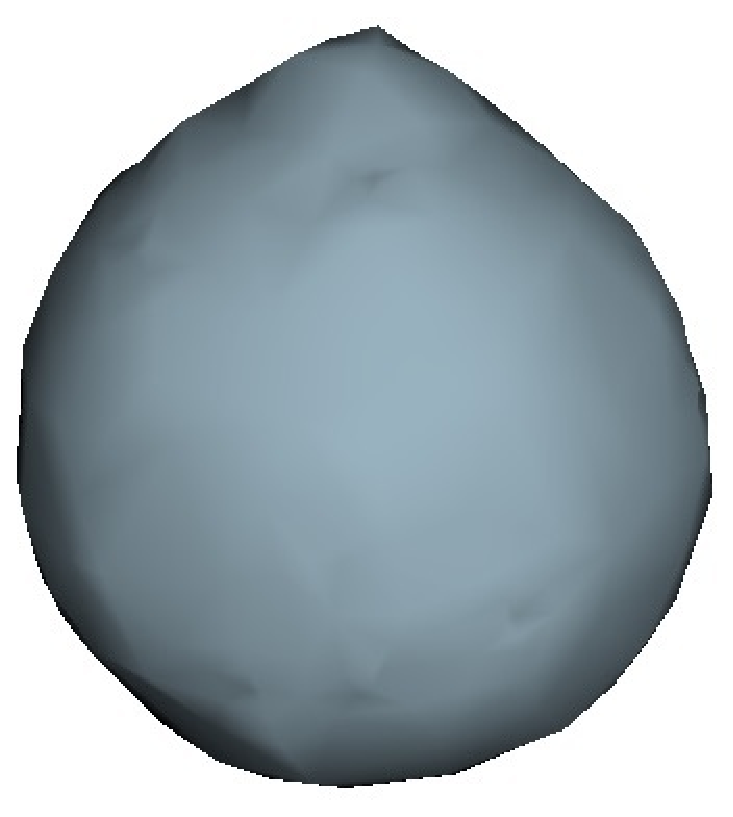
\includegraphics[width=0.30\columnwidth]{deformedspherepoisson.eps}
}
\caption{Deformed sphere using (from left to right): the HRBF approach, 
the closed form solution to the HRBF approach and the Poisson surface
reconstruction approach}
\end{figure} 
\end{frame}

\begin{frame}
\frametitle{Example of sculpture}
\Large
\begin{figure}
  \centering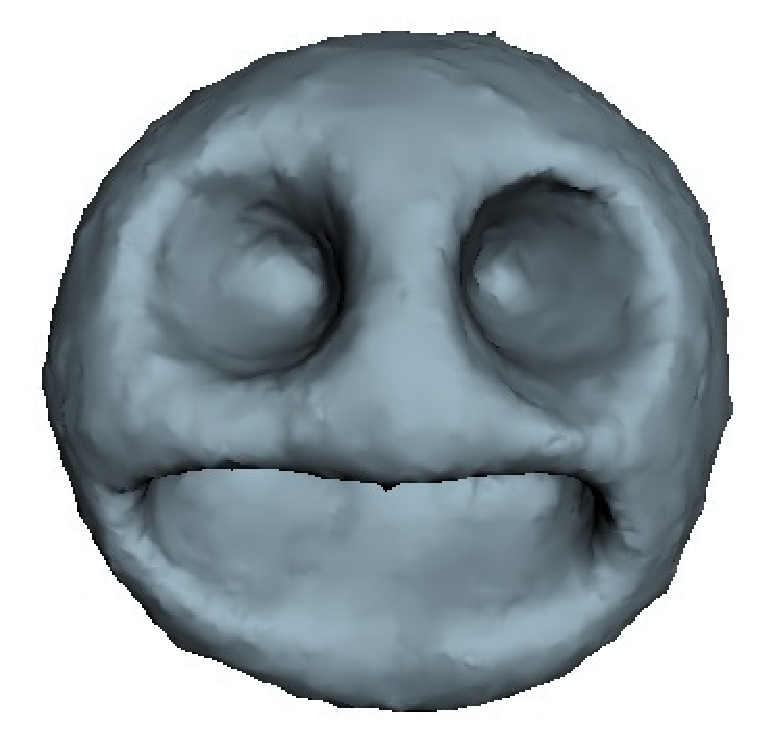
\includegraphics[width=0.3\columnwidth]{simplefacepoisson2.eps}
  \caption{Example to model a simple character face} \label{fig:face}
\end{figure}
\begin{itemize}
\item The eyes and the mouth were carved by changing the sign of the field used for the deformation.
\item Changing the width of the Gaussian function used for the deformation could allow to add or carve smaller details.
\end{itemize}
\end{frame}

\begin{frame}
\frametitle{Deformation of a more complex surface}
\begin{figure}
  \centering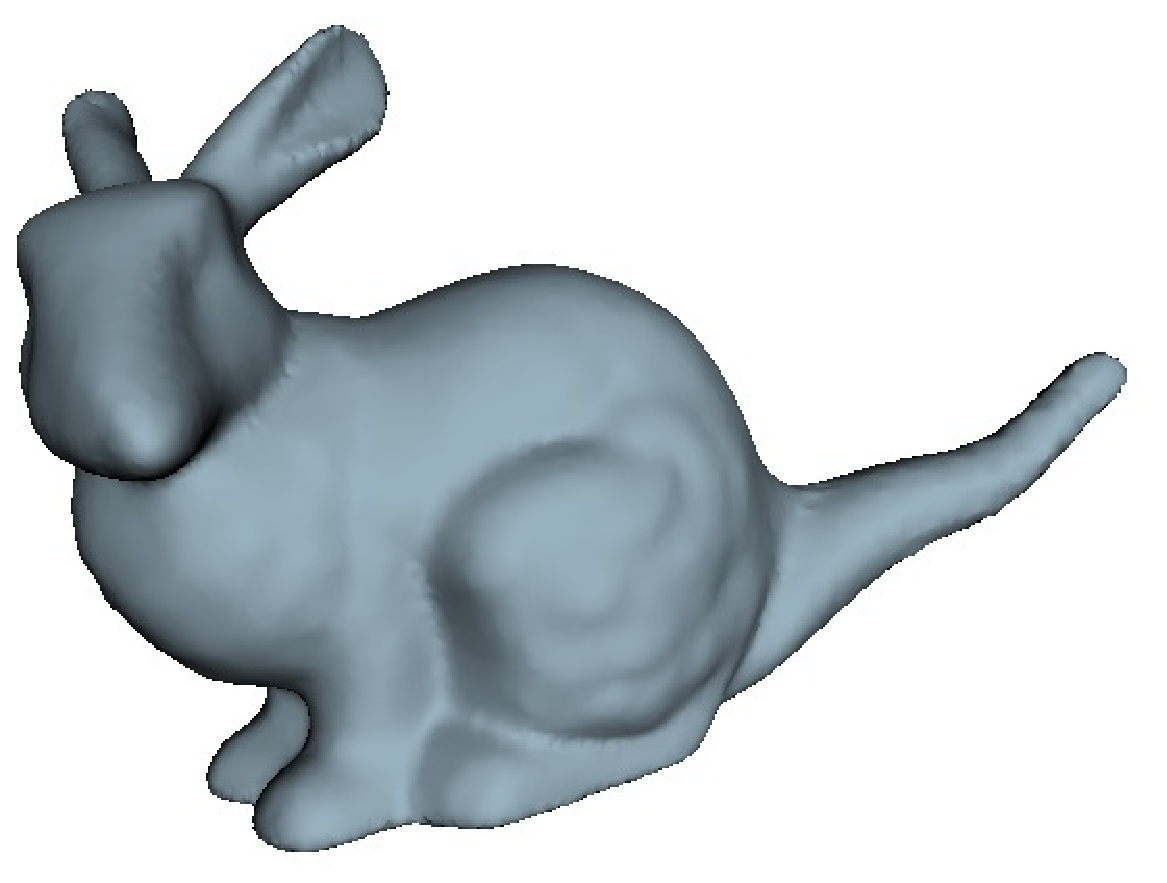
\includegraphics[width=0.4\columnwidth]{deformedbunnypoisson.eps}
  \caption{Deformed bunny object with stretched tail and nose} \label{fig:bunnyPoisson}
\end{figure}

\Large
\begin{itemize}
\item The input mesh for this object contains 14072 vertices and 28042 triangles.
\item  Both the tail and the nose are stretched.
\end{itemize}


\end{frame}
\section{Conclusion}
\begin{frame}
\frametitle{Conclusion}
\Large
\begin{itemize}
\item A simple algorithm for mesh deformation.
\item Sample from the mesh, deforms the sample (no connectivity to maintain), perform surface
reconstruction.
\item Future works : algorithmitic improvements, implementation of parts of the algorithm on the graphics card (GPU).
\end{itemize}
\end{frame}
\begin{frame}
\frametitle{ {\color{blue}.}}
\centering
\Large
Thank you.

\end{frame}


\end{document}
